\documentclass[12pt,a4paper]{article}

\usepackage[UTF8]{ctex}
\usepackage{amsmath,amscd,amsbsy,amssymb,latexsym,url,bm,amsthm}
\usepackage{amsfonts}
\usepackage{epsfig,graphicx,subfigure}
\usepackage{hyperref}
\usepackage{listings}
\usepackage[vlined,ruled,linesnumbered]{algorithm2e}
\usepackage{enumitem}
\usepackage{xcolor}
\usepackage{geometry}

%\uppercase\expandafter{\romannumeral1}:% 罗马数字。

\lstset{
language=Matlab,
keywordstyle= \color{blue!70},
commentstyle= \color{red!50!green!50!blue!50},
breaklines
}%设置listing插入语言

\setlength{\parindent}{0em}
\setlength{\parskip}{1em}

\geometry{bottom =3cm}
\newcommand{\textbi}[1]{%
\textbf{\textit{#1}}}

\newcommand{\ncolor}[1]{%
{\color[RGB]{139,117,0}{#1}}}
\newtheorem{theorem}{Theorem}[section]
\newenvironment{solution}{{\noindent \it \textbf{Solution:}}\\}

\title{MCM daily}
\author{Yunlong Cheng}

\begin{document}
\maketitle

\section{Model learning}
\subsection{非线性规划}
\subsubsection{非线性规划的MATLAB解法}

\begin{equation*}
  \begin{split}
    minimize\quad & f(x)\\
    subject\;to &\\
    \mathbf{Ax}& \le \mathbf{B}\\
    Aeq \cdot \mathbf{x}& = Beq\\
    \mathbf{C(x)}& \le 0\\
    Ceq(\mathbf{x})& = 0
  \end{split}
\end{equation*}
使用命令:
\begin{lstlisting}
  X = FMINCON(FUN,X0,A,B,Aeq,Beq,LB,UB,NONLCON,OPTIONS)
\end{lstlisting}
例:
\begin{equation*}
  \begin{split}
    min f(x)& = x_1^2+x_2^2+8\\
    subject\;to&\\
    x_1^2-x_2& \ge 0\\
    -x_1-x_2^2+2& = 0\\
    x_1, x_2& \ge 0
  \end{split}
\end{equation*}
解:\href{run:matlab/fun1.m}{fun1.m}, \href{run:matlab/fun2.m}{fun2.m}.

\subsection{二次规划}
目标函数为自变量x的二次函数,约束条件全是线性的。
使用命令:
\begin{lstlisting}
[X,FVAL] = QUADPROG(H,f,A,b,Aeq,beq,LB,UB,X0,OPTIONS)
\end{lstlisting}
利用到线性代数中的二次型。

\subsection*{罚函数法}
利用不等式构造带参数的增广目标函数,将问题转化为无约束非线性规划问题。

\subsection{整数规划}
\subsubsection{求解方法}
\begin{enumerate}
  \item 分枝定界法
  \item 割平面法
  \item 隐枚举法
  \item 匈牙利法
  \item 蒙特卡洛法
\end{enumerate}
老老实实用LINGO。

\subsection{灰色预测与模型}
通过对原始数据进行整理,变成有规律的时间序列数据,再建立动态模型。常用的数据处理方式有两种:累加和累减,通常用累加。

灰色模型中,以灰色系统中单序列一阶线性微分方程模型$GM(1,1)$模型最为常用。
\subsubsection{GM(1,1) 模型}
原始数据列:
$$x^{(0)} = (x^{(0)}(1), x^{(0)}(2),\cdots ,x^{(0)}(n))$$
基本步骤:
\begin{enumerate}
  \item [(1)] 得到新数据序列 $x^{(1)}(t)$
  \item [(2)] 建立新数据序列的一阶微分方程:
  $$\frac{dx^{(1)}}{dt}+ax^{(1)} = u$$
  $\hat a = \binom a u$
  \item [(3)] 对累加生成数据做均值生成 $B$ 与常数项向量 $Y_n$ 。
  \begin{equation*}
    \mathbf{B} = \left[
    \begin{array}{c}
      0.5(x^{(1)}(1)+x^{(1)}(2))\\
      0.5(x^{(1)}(2)+x^{(1)}(3))\\
      \cdots \\
      0.5(x^{(1)}(n-1)+x^{(1)}(n))\\
    \end{array} \right],
    \mathbf{Y_n} = (x^{(0)}(2),x^{(0)}(3) ,\cdots, x^{(0)}(n))^T
  \end{equation*}
  \item [(4)] 用最小二乘法求解灰参数 $\hat a$.
  \item [(5)] 将灰参数 $\hat a$ 带入求解。
  $$\hat x ^{(1)}(t+1)=(\hat x^{(0)}(1) - \frac{u}{a})e^{-at} + \frac{u}{a}$$
  \item [(6)] 对 $\hat x ^{(1)}(t+1)$ 及 $\hat x ^{(1)}(t)$ 进行离散。
  \item [(7)] 检验灰色模型。
  \item [(8)] 利用模型进行预测。
\end{enumerate}


\section{Algorithm learning}
\subsection{遗传算法(Genetic algorithm)}
\subsubsection{编码}
二进制编码:
设某一参数取值范围为$(L,U)$,使用长度为 $k$ 的二进制编码表示该参数。
\begin{center}
  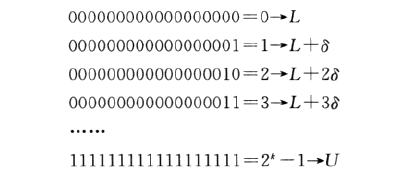
\includegraphics[width=0.7\textwidth]{figures/encoding}
\end{center}
易知:
$$\delta = \frac{U-L}{2^k-1}$$
\subsubsection{解码}
$$x = L + (\sum_{i = 1}^kb_i2^{i-1})\frac{U-L}{2^k-1}$$
\subsubsection{交配}
用随机数产生一个或多个交配点位置,然后两个个体在交配点位置互换部分基因码,形成两个子个体。
\subsubsection{突变}
“突变运算”是使用基本位进行基因突变。对于二进制的基因码组成的个体种群,实行基因码的小几率翻转,对于二进制编码即 0 变为 1 ,而 1 变为 0 。
\subsubsection{倒位}
倒位是指一个染色体某区段正常排列顺序发生180°的颠倒,造成染色体内的 DNA 序列重新排列,它包括臂内倒位和臂间倒位。
\subsubsection{个体适应度评估}
\subsubsection{复制}
复制运算是根据个体适应度大小决定其下代遗传的可能性。若设种群中个体总数为 $N$ ,个体 $i$ 的适应度为 $f$ ,则个体 $i$ 被选取的几率:
$$P_i = \frac{f_i}{\sum_{k = 1}^{N}f_k}$$
\subsubsection{拓展:协同进化遗传算法}
\newpage
\subsubsection{Matlab实现}
伪代码:

\begin{minipage}[t]{0.9\textwidth}
  \begin{algorithm}[H]
    \BlankLine
    \caption{pseudo code for Genetic algorithm}
    $t\leftarrow 0$\;
    初始化P(t)\;
    计算P(t)的适应值\;
    \While{不满足准则}{
      $t\leftarrow t + 1$\;
      从P(t-1)中选择P(t)\;
      重组P(t)\;
      计算P(t)的适应值\;
    }
  \end{algorithm}
\end{minipage}

安装 Global Optimization Toolbox.
\href{run:matlab/P4-1/GA401.m}{GA401.m}\\
多约束非线性规划问题可以用 GA 和 Lingo 求解。
\end{document}
